\documentclass[11pt]{article}
\usepackage[margin=1in]{geometry}
\usepackage{amsmath,amssymb,booktabs,graphicx,setspace,caption,hyperref}
\usepackage[T1]{fontenc}
\usepackage{mathpazo}
\setlength{\parindent}{0pt}
\setlength{\parskip}{0.6em}
\captionsetup{font=small,skip=6pt}
\title{Panel MS-AR(1) with quarterly dummies, 1995Q1 onward\\[0.4em]\large Real GDP per worker (period-average USD)}
\author{}
\date{}
\begin{document}
\maketitle
\section{Model}
Joint panel Markov-switching AR(1) around a linear trend with common quarterly dummies (Q1 omitted):
\begin{align}
y_{it} &= a_i + g\, t + d_2 Q2_t + d_3 Q3_t + d_4 Q4_t + z_{it}, \\
z_{i,t+1} &= \bigl(1-\rho(s_{it})\bigr)\mu(s_{it}) + \rho(s_{it})\, z_{it} + \sigma(s_{it})\,\varepsilon_{it}, \\
s_{i,t+1} &\sim \Pi(\,\cdot\mid s_{it}).
\end{align}
The sample is restricted to calendar time from 1995Q1. Specification 1 sets $a_i\equiv a$. Specification 2 lets $a_i\sim\mathcal{N}(\alpha,\omega^2)$, integrating each country by 11-point Gauss--Hermite. The slope $g$ and the quarterly dummies are common. $|\rho|<0.99$. Median $\mu$ pinned at 0. Cycles use posterior-mean $a_i$ in the RE specification. Standard errors are delta-method from a numerical Hessian.
\clearpage
\section{Common intercept, linear trend, and quarterly dummies}
2026-09-14 panel from 1995Q1: log real GDP per worker. 90 countries, 7975 observations, 1995-Q1--2026-Q2. Fitted countries: 90. Observations: 7975. Log-likelihood: 12436.63. Ergodic mean of the cycle $E[z]=0.4724$ (0.0941).
Common intercept $a=-5.4017$ (0.0771). Common slope $g=-0.0018$ (0.0016). Seasonal dummies (Q1 omitted): $d_{Q2}=0.0177$ (0.0009), $d_{Q3}=0.0128$ (0.0010), $d_{Q4}=0.0432$ (0.0009).
\begin{table}[h]
\centering
\caption{Regime AR(1), transition matrix, and ergodic $\pi$. Columns are regimes.}
\begin{tabular}{lccc}
\toprule
 & (0) & (1) & (2) \\
\midrule
$\mu$ & -1.1440 & 0.0000 & 1.5060 \\
 & (0.3007) & --- & (0.0708) \\ \addlinespace
$\sigma$ & 0.1693 & 0.0654 & 0.0274 \\
 & (0.0050) & (0.0013) & (0.0005) \\ \addlinespace
$\rho$ & 0.9900 & 0.9900 & 0.9900 \\
 &  & (0.0000) & (0.0000) \\ \addlinespace
$\Pi_{0\cdot}$ & 0.9825 & 0.0149 & 0.0026 \\
 & (0.0060) & (0.0050) & (0.0032) \\ \addlinespace
$\Pi_{1\cdot}$ & 0.0039 & 0.9808 & 0.0153 \\
 & (0.0013) & (0.0029) & (0.0026) \\ \addlinespace
$\Pi_{2\cdot}$ & 0.0015 & 0.0158 & 0.9827 \\
 & (0.0012) & (0.0026) & (0.0023) \\ \addlinespace
$\pi$ & 0.1357 & 0.4474 & 0.4169 \\
 & (0.0289) & (0.0354) & (0.0363) \\ \addlinespace
\bottomrule
\end{tabular}
\end{table}
\begin{figure}[h]
\centering
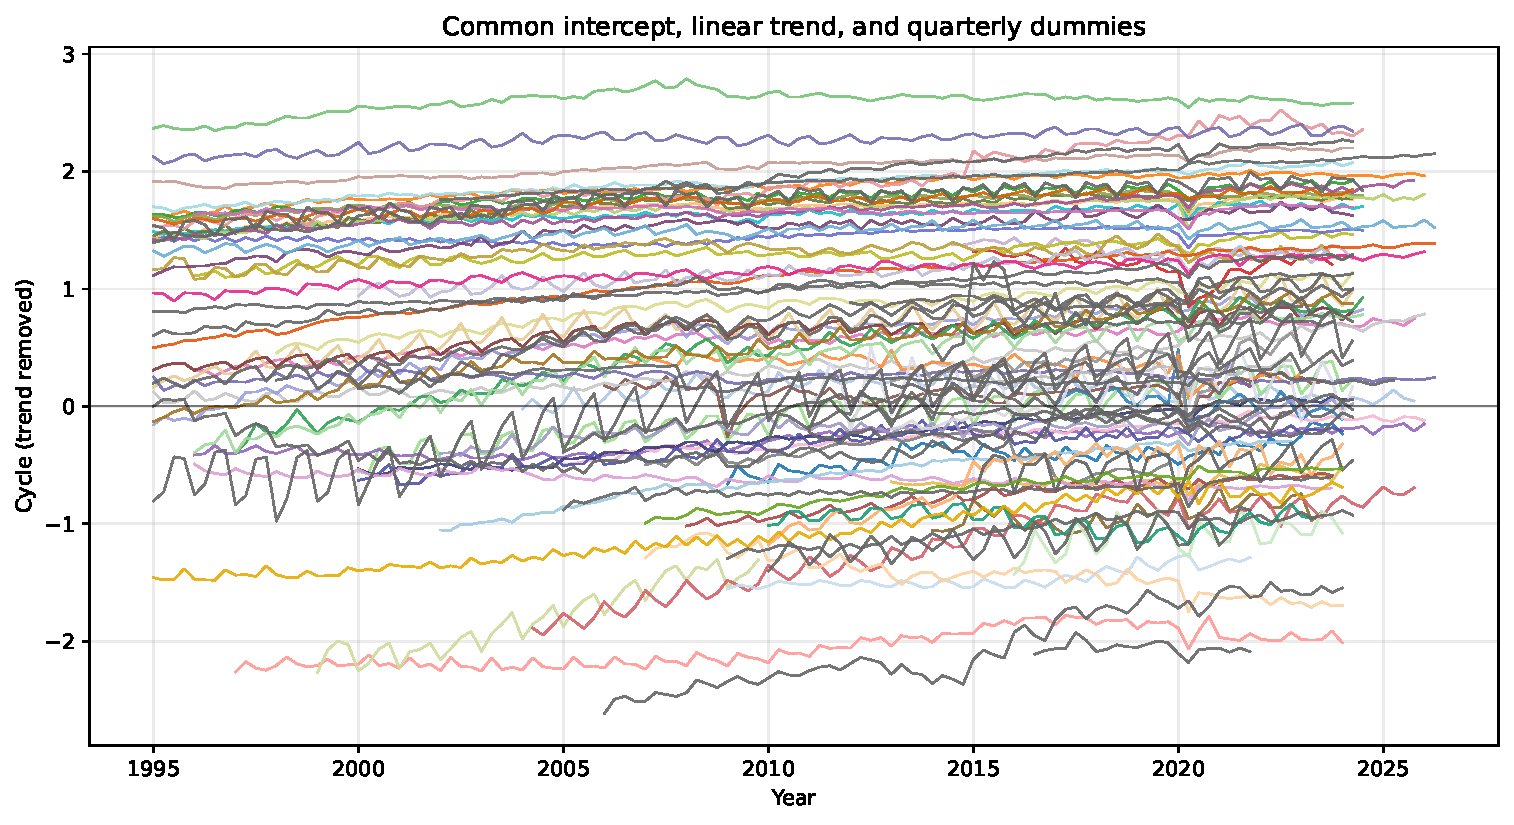
\includegraphics[width=0.75\textwidth]{figs/cycle_common_ag_q_1995.pdf}
\caption{Country cycles after removing the linear trend and quarterly means.}
\end{figure}
\clearpage
\section{RE intercepts, common trend and quarterly dummies}
2026-09-14 panel from 1995Q1: log real GDP per worker. 90 countries, 7975 observations, 1995-Q1--2026-Q2. Fitted countries: 90. Observations: 7975. Log-likelihood: 12732.16. Ergodic mean of the cycle $E[z]=-0.0437$ (0.0442).
Random intercepts $a_i\sim N(\alpha,\omega^2)$ with $\alpha=-5.4306$ (0.0822), $\omega=0.7551$ (0.0255). Posterior-mean $a_i$: mean -5.362, min -7.603, max -3.267. Common slope $g=0.0166$ (0.0013). Seasonal dummies (Q1 omitted): $d_{Q2}=0.0180$ (0.0008), $d_{Q3}=0.0126$ (0.0009), $d_{Q4}=0.0422$ (0.0008).
\begin{table}[h]
\centering
\caption{Regime AR(1), transition matrix, and ergodic $\pi$. Columns are regimes.}
\begin{tabular}{lccc}
\toprule
 & (0) & (1) & (2) \\
\midrule
$\mu$ & -0.2568 & 0.0000 & 0.0408 \\
 & (0.0834) & --- & (0.0899) \\ \addlinespace
$\sigma$ & 0.1582 & 0.0645 & 0.0260 \\
 & (0.0045) & (0.0012) & (0.0004) \\ \addlinespace
$\rho$ & 0.6745 & 0.9748 & 0.9898 \\
 & (0.0356) & (0.0043) & (0.0004) \\ \addlinespace
$\Pi_{0\cdot}$ & 0.9814 & 0.0121 & 0.0065 \\
 & (0.0061) & (0.0051) & (0.0049) \\ \addlinespace
$\Pi_{1\cdot}$ & 0.0032 & 0.9844 & 0.0125 \\
 & (0.0011) & (0.0028) & (0.0026) \\ \addlinespace
$\Pi_{2\cdot}$ & 0.0018 & 0.0114 & 0.9868 \\
 & (0.0010) & (0.0022) & (0.0020) \\ \addlinespace
$\pi$ & 0.1168 & 0.4243 & 0.4589 \\
 & (0.0260) & (0.0382) & (0.0391) \\ \addlinespace
\bottomrule
\end{tabular}
\end{table}
\begin{figure}[h]
\centering
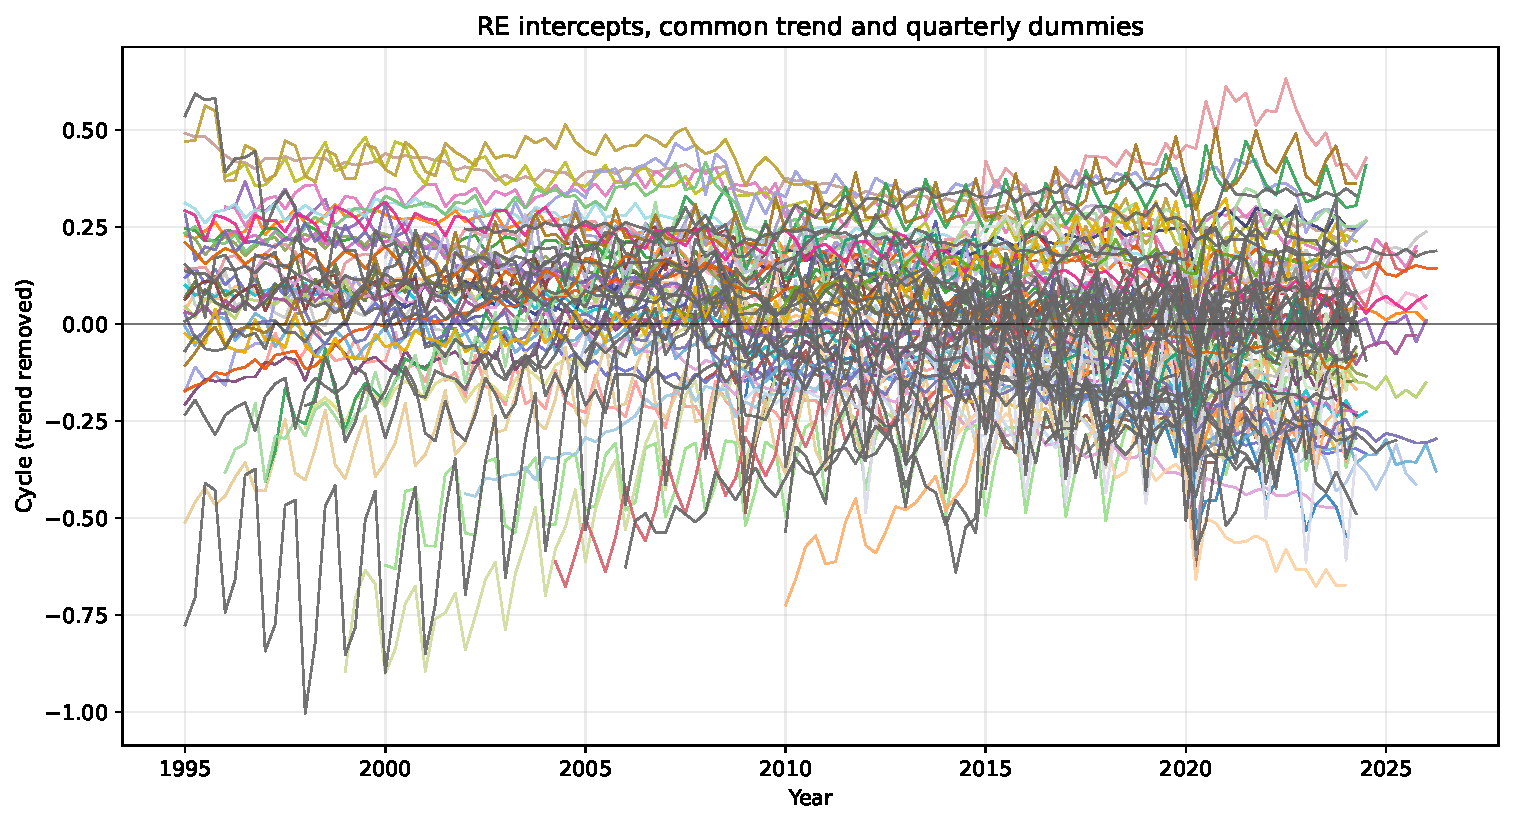
\includegraphics[width=0.75\textwidth]{figs/cycle_re_ai_q_1995.pdf}
\caption{Country cycles after removing the linear trend and quarterly means.}
\end{figure}
\end{document}
